\documentclass{article}
\usepackage{graphicx} % Required for inserting images
\usepackage[utf8]{inputenc}
\usepackage{setspace}
\usepackage[margin=1.5cm]{geometry}
\usepackage{amsmath}
\usepackage{amsthm}
\usepackage{amsfonts}
\usepackage{indentfirst}
\usepackage{tikz}

\title{Integrating over Regions}
\author{Matthew Seguin}
\date{}

\begin{document}

\maketitle

\section*{49.1}
\begin{center}
    \doublespacing
    Recall that if a continuous function $f$ has an antiderivative $F$ throughout a domain $D$ then for any contour $C$ going from $z_1$ to $z_2$ contained in $D$ we know:
    \[\int _C f(z)dz = F(z)\Big{|}_{z_1}^{z_2}\]
    Now let's look at $f(z) = z^n$ where $n\in\{0, 1, 2, ...\}$.
    \\We have seen before that for $n\in\mathbb{Z}\backslash\{0\}$ that $\frac{d}{dz} z^n = nz^{n-1}$, therefore we can apply this to $n\in\{1, 2, 3, ...\}$.
    \\So we have that $\frac{d}{dz}\frac{z^n}{n} = z^{n-1}$ for all $n\in\{1, 2, 3, ...\}$.
    \\Then letting $m = n - 1$ we see that $n = m + 1$ and $\frac{d}{dz}\frac{z^{m+1}}{m+1} = z^m$ where $m\in\{0, 1, 2, ...\}$.
    \\Therefore for all $m\in\{0, 1, 2, ...\}$ we have that the antiderivative of $z^m$ is $\frac{z^{m+1}}{m+1}$.
    \break
    \\Recall that $z^m$ is entire for all $m\in\{0, 1, 2, ...\}$.
    \\This means that for all $m\in\{0, 1, 2, ...\}$ we know that for any contour $C$ going from $z_1$ to $z_2$:
    \[\int _C z^m dz =\frac{z^{m+1}}{m+1}\Big{|}_{z_1}^{z_2} =\frac{1}{m+1}\big{(}z_2^{m+1} - z_1^{m+1}\big{)}\]
    \qedsymbol
\end{center}


\newpage
\section*{49.3}
\begin{center}
    \doublespacing
    Recall that if a continuous function $f$ has an antiderivative $F$ throughout a domain $D$ then for any contour $C$ going from $z_1$ to $z_2$ contained in $D$ we know:
    \[\int _C f(z)dz = F(z)\Big{|}_{z_1}^{z_2}\]
    We have seen before that for $n\in\mathbb{Z}\backslash\{0\}$ that $\frac{d}{dz} z^n = nz^{n-1}$.
    \\Therefore we know that $\frac{d}{dz}\frac{z^n}{n} = z^{n-1}$ for all $n\in\mathbb{Z}\backslash\{0\}$.
    \break
    \\If a contour $C_0$ does not pass through $z_0$ then we know that for each $z\in C_0$ there must exist some neighborhood where $z_0\notin V_{\epsilon _z} (z)$ for every point $z\in C_0$.
    \\So there must exist some domain $D_0$ (which can be the union of all these neighborhoods) that contains $C_0$ and not $z_0$.
    \\Therefore for $n\in\{\pm 1,\pm 2, \pm 3, ...\}$ we know $(z - z_0)^{n-1}$ is continuous and has an antiderivative on $D_0$ (negative powers aren't a problem since $z\neq z_0$).
    \break
    \\Therefore for any contour $C_0$ going from $z_1$ to $z_2$ that does not pass through $z_0$ we may say that for $n\in\{\pm 1,\pm 2,\pm 3, ...\}$:
    \[\int _{C_0} (z - z_0)^{n-1} dz =\frac{(z - z_0)^n}{n}\Big{|}_{z_1}^{z_2} =\frac{1}{n}\Big{(}(z_1 - z_0)^n - (z_2 - z_0)^n\Big{)}\]
    Therefore if $C_0$ is a closed contour (i.e. $z_1 = z_2 = z$) that does not pass through $z_0$ we may say that for $n\in\{\pm 1,\pm 2,\pm 3, ...\}$:
    \[\int _{C_0} (z - z_0)^{n-1} dz =\frac{(z - z_0)^n}{n}\Big{|}_{z_1}^{z_2} =\frac{1}{n}\Big{(}(z_1 - z_0)^n - (z_2 - z_0)^n\Big{)} = \frac{1}{n}\Big{(}(z - z_0)^n - (z - z_0)^n\Big{)} = 0\]
    \qedsymbol
\end{center}


\newpage
\section*{49.4}
\begin{center}
    \doublespacing
    Let $f_2 (z)$ be the branch $f_2 (z) =\sqrt{r} e^{i\frac{\theta}{2}}$ of $z^{\frac{1}{2}}$ where $\frac{\pi}{2}\leq\theta\leq\frac{5\pi}{2}$.
    \\Then let $C_2$ be the contour as shown in the example (although the exact shape doesn't matter) which goes from $-3$ to 3.
    \break
    \\Now consider the function $F_2 (z) =\frac{2}{3} z^{\frac{3}{2}} =\frac{2}{3}\sqrt{r^3} e^{i\frac{3\theta}{2}} =\frac{2}{3} r^{\frac{3}{2}}(cos(\frac{3\theta}{2}) + i\:sin(\frac{3\theta}{2}))$ with the same bounds on $\theta$.
    \\Then we can write $F_2 (z) = u(r,\theta) + iv(r,\theta)$ where $u(r,\theta) =\frac{2}{3} r^{\frac{3}{2}} cos(\frac{3\theta}{2})$ and $v(r,\theta) =\frac{2}{3} r^{\frac{3}{2}} sin(\frac{3\theta}{2})$.
    \\Looking at the partial derivatives:
    \\$u_r =r^{\frac{1}{2}} cos(\frac{3\theta}{2})$, $u_{\theta} = -r^{\frac{3}{2}} sin(\frac{3\theta}{2})$, $v_r = r^{\frac{1}{2}} sin(\frac{3\theta}{2})$, $v_{\theta} = r^{\frac{3}{2}} cos(\frac{3\theta}{2})$
    \\Clearly $r u_r = r^{\frac{3}{2}} cos(\frac{3\theta}{2}) = v_{\theta}$ and $u_{\theta} = -r^{\frac{3}{2}} sin(\frac{3\theta}{2}) = -r(r^{\frac{1}{2}} sin(\frac{3\theta}{2})) = -r v_r$.
    \\So the polar Cauchy Riemann equations are satisfied.
    \\Furthermore the partial derivatives are continuous so we know that $F_2 (z)$ is differentiable and $F_2 '(z) = e^{-i\theta} (u_r + iv_r)$.
    \\So $F_2 '(z) = e^{-i\theta} (r^{\frac{1}{2}} (cos(\frac{3\theta}{2}) + i r^{\frac{1}{2}} sin(\frac{3\theta}{2})) = r^{\frac{1}{2}} e^{-i\theta} e^{i\frac{3\theta}{2}} =\sqrt{r} e^{i\frac{\theta}{2}} = f_2 (z)$ since they have the same $\theta$ bounds.
    \\So $F_2 (z) =\frac{2}{3} z^{\frac{3}{2}} =\frac{2}{3}\sqrt{r^3} e^{i\frac{3\theta}{2}}$ is an antiderivative for $f_2 (z)$.
    \break
    \\Therefore we know:
    \[\int _{C_2} f_2 (z) dz = F_2 (z)\Big{|}_{-3}^3 =\frac{2}{3}\sqrt{27} (e^{i\frac{3(2\pi)}{2}} - e^{i\frac{3(\pi)}{2}}) = 2\sqrt{3} (e^{3i\pi} - e^{i\frac{3\pi}{2}}) = 2\sqrt{3} (-1 + i)\]
    \qedsymbol
    \\Note then that:
    \[\int _{C_2 - C_1} z^{\frac{1}{2}} dz =\int _{C_2} f_2 (z) dz -\int _{C_1} f_1 (z) dz = 2\sqrt{3}(-1 + i) - 2\sqrt{3}(1 + i) = -4\sqrt{3}\]
\end{center}


\newpage
\section*{53.1}

{\Large\textbf{c.}} Let $f(z) =\frac{1}{z^2 + 2z + 2}$ and let $C$ be the unit circle $|z| = 1$.
\begin{center}
    \doublespacing
    We know we can solve for the roots of $z^2 + 2z + 2$ with the quadratic equation, as shown in a previous sample work.
    \\So $z =\frac{-2\pm\sqrt{2^2 - 4(1)(2)}}{2} =\frac{-2\pm\sqrt{-4}}{2} =\frac{-2\pm 2i}{2} = -1\pm i$.
    \\Clearly neither of these roots are interior to or on the contour $C$, this can be easily shown by noticing $|-1\pm i| =\sqrt{(-1)^2 + (\pm 1)^2} =\sqrt{2} > 1$.
    \\Recall both polynomials and constant functions are entire, and therefore analytic at all points interior to and on $C$.
    \break
    \\So since $P(z) = z^2 + 2z + 2$ and $g(z) = 1$ are analytic at all points interior to and on $C$, and since $P(z)\neq 0$ for any point interior to or on $C$ we know that $f(z) =\frac{1}{z^2 + 2z + 2} =\frac{g(z)}{P(z)}$ is analytic at all points interior to and on $C$.
    \\Therefore since $C$ is a simple closed contour (being just the unit circle $|z| = 1$) we may use the Cauchy-Goursat Theorem.
    \\So we have that:
    \[\int _C f(z) dz =\int _C\frac{1}{z^2 + 2z + 2} dz = 0\]
    Notice that the direction of $C$ was unspecified and the integral still evaluates to 0, this is because no matter the direction it is still a simple closed contour.
    \\ \qedsymbol
\end{center}


\newpage
\section*{53.2}

{\Large\textbf{b.}} Let $f(z) =\frac{z + 2}{sin(\frac{z}{2})}$.
\begin{center}
    \doublespacing
    Then let $C_1$ be the positively oriented unit square whose sides lie on $x =\pm 1$ and $y =\pm 1$ and $C_2$ be the positively oriented circle $|z| = 4$.\\
    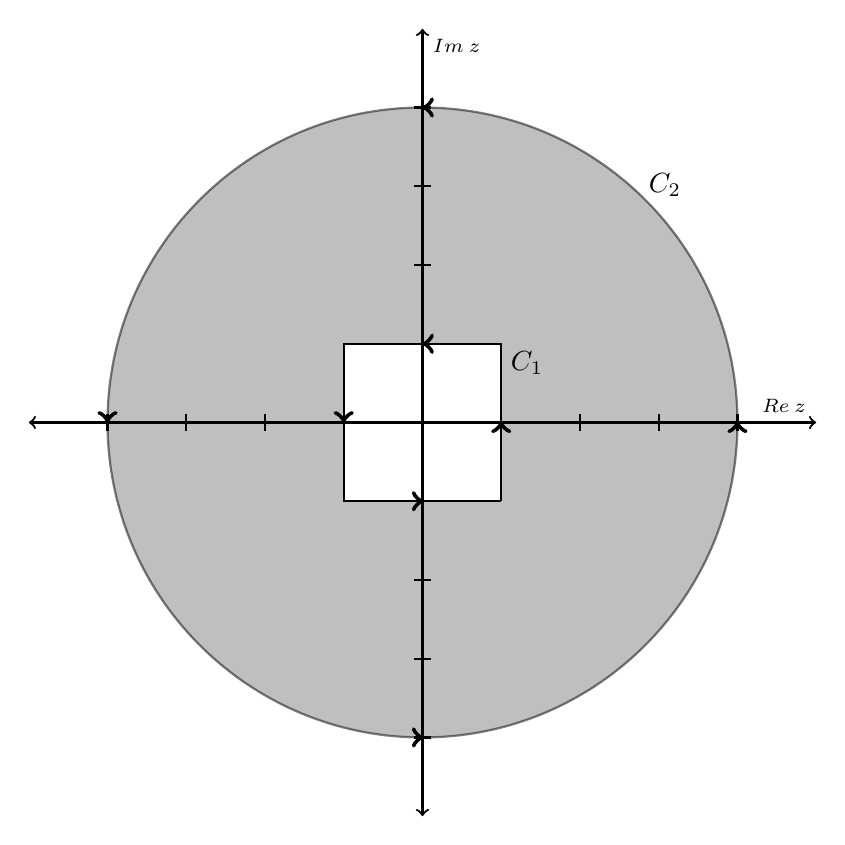
\begin{tikzpicture}
    \begin{scope}[thick,font=\scriptsize]
    \path [draw=black,fill=gray,semitransparent] (0,0) circle (4);
    \draw [line width=0.25mm,fill=white] (1,-1) -- (1,1) -- (-1,1) -- (-1,-1) -- (1,-1);
    \draw [<->] (-5,0) -- (5,0) node [above left]  {$Re\:z$};
    \draw [<->] (0,-5) -- (0,5) node [below right] {$Im\:z$};
    \foreach \n in {-4,...,-1,1,2,...,4}{
        \draw (\n,-3pt) -- (\n,3pt);
        \draw (-3pt,\n) -- (3pt,\n);
    }
    \end{scope}
    \draw [->,ultra thick] (4,0) -- (4,0.01);
    \draw [->,ultra thick] (-4,0.01) -- (-4,0);
    \draw [->,ultra thick] (0,-4) -- (0.01,-4);
    \draw [->,ultra thick] (0.01,4) -- (0,4);
    \draw [->,ultra thick] (1,0) -- (1,0.01);
    \draw [->,ultra thick] (-1,0.01) -- (-1,0);
    \draw [->,ultra thick] (0,-1) -- (0.01,-1);
    \draw [->,ultra thick] (0.01,1) -- (0,1);
    \node [above right, black] at (2.75,2.75) {$C_2$};
    \node [right, black] at (1,0.75) {$C_1$};
    \end{tikzpicture}
    \\Clearly $C_1$ is interior to $C_2$.
    \\Furthermore since $sin(\frac{z}{2}) = 0$ if and only if $\frac{z}{2} = n\pi$ and hence only if $z = 2n\pi$ for some $n\in\mathbb{Z}$ we know that $sin(\frac{z}{2})\neq 0$ for any point lying on or in between the contours $C_1$ and $C_2$.
    \\This is because for $n\in\mathbb{Z}\backslash\{0\}$ we know $|\pm 2n\pi| = 2n\pi\geq 2\pi = |\pm 2\pi|$ and clearly $2\pi > 4$ so all of these points lie outside of the region between $C_1$ and $C_2$. Also, as clearly seen above $z = 0$ is not on or lying between the contours $C_1$ and $C_2$.
    \break
    \\Recall that polynomials and $sin(w)$ are entire, therefore we have that $g(z) = sin(\frac{z}{2})$ and $P(z) = z + 2$ are analytic on and between the contours $C_1$ and $C_2$.
    \\Since $sin(\frac{z}{2})\neq 0$ on or between the contours $C_1$ and $C_2$ we know $f(z) =\frac{z + 2}{sin(\frac{z}{2})} =\frac{P(z)}{g(z)}$ is analytic on and between the contours $C_1$ and $C_2$.
    \\Therefore since $C_1$ and $C_2$ are positively oriented simple closed contours where $C_1$ is interior to $C_2$ and we know $f(z) =\frac{z + 2}{sin(\frac{z}{2})}$ is analytic on and between the contours $C_1$ and $C_2$ we may use the corollary in the book to say:
    \[\int _{C_1} f(z) dz =\int _{C_1}\frac{z + 2}{sin(\frac{z}{2})} dz =\int _{C_2}\frac{z + 2}{sin(\frac{z}{2})} dz =\int _{C_2} f(z) dz\]
    \qedsymbol
\end{center}


\newpage
\section*{53.3}
\begin{center}
    \doublespacing
    Let $C$ be the boundary of the rectangle $0\leq x\leq 3$ and $0\leq y\leq 2$ taken in the positive orientation.
    \\Now let $C_0$ be the boundary of the circle $|z - (2 + i)| = 3$ taken in the positive orientation.
    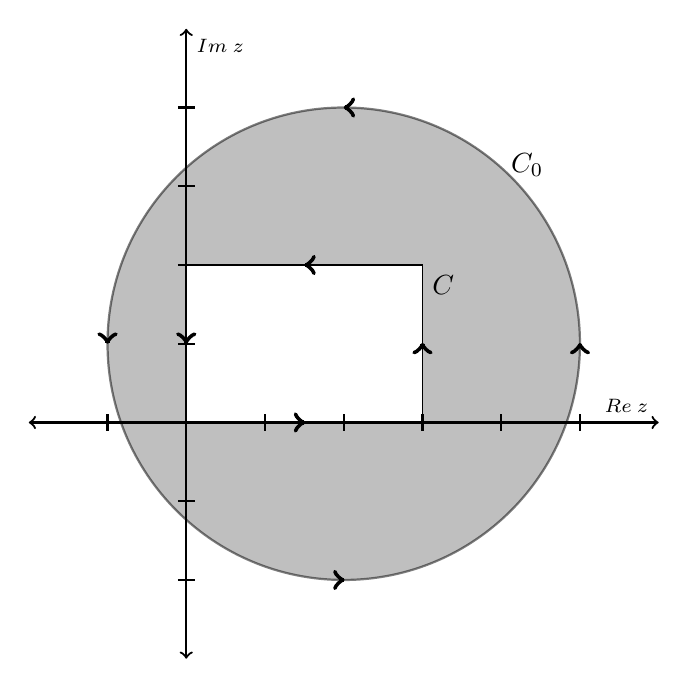
\begin{tikzpicture}
    \begin{scope}[thick,font=\scriptsize]
    \path [draw=black,fill=gray,semitransparent] (2,1) circle (3);
    \draw [line width=0.25mm,fill=white] (0,0) -- (3,0) -- (3,2) -- (0,2) -- (0,0);
    \draw [<->] (-2,0) -- (6,0) node [above left]  {$Re\:z$};
    \draw [<->] (0,-3) -- (0,5) node [below right] {$Im\:z$};
    \foreach \n in {-1,...,-1,1,2,...,5}{
        \draw (\n,-3pt) -- (\n,3pt);
    }
    \foreach \n in {-2,...,-1,1,2,...,4}{
        \draw (-3pt,\n) -- (3pt,\n);
    }
    \end{scope}
    \draw [->,ultra thick] (3,1) -- (3,1.01);
    \draw [->,ultra thick] (0,1.01) -- (0,1);
    \draw [->,ultra thick] (1.5,0) -- (1.51,0);
    \draw [->,ultra thick] (1.51,2) -- (1.5,2);
    \draw [->,ultra thick] (5,1) -- (5,1.01);
    \draw [->,ultra thick] (-1,1.01) -- (-1,1);
    \draw [->,ultra thick] (2,-2) -- (2.01,-2);
    \draw [->,ultra thick] (2.01,4) -- (2,4);
    \node [above right, black] at (4,3) {$C_0$};
    \node [right, black] at (3,1.75) {$C$};
    \end{tikzpicture}
    \\Clearly $C$ is interior to $C_0$.
    \\Since polynomials are entire we have that $z - (2 + i)$ is analytic on and between the contours $C$ and $C_0$.
    \\Furthermore we know that $z - (2 + i)\neq 0$ for any $z$ lying on or between the contours $C$ and $C_0$.
    \\Consequently $(z - (2 + i))^{n-1}$ is analytic on and between the contours $C$ and $C_0$ for any $n\in\mathbb{Z}$ (since $z - (2 + i)\neq 0$ for any $z$ on or between the contours $C$ and $C_0$ negative powers are not a problem).
    \\Therefore since $C$ and $C_0$ are positively oriented simple closed contours where $C$ is interior to $C_0$ and we know $(z - (2 + i))^{n-1}$ is analytic on and between the contours $C$ and $C_0$ we may use the corollary in the book to say:
    \[\int _{C} (z - (2 + i))^{n-1} dz =\int _{C_0} (z - (2 + i))^{n-1} dz\]
    \\Recall from problem in a previous sample work that when $C_0$ denotes the positively oriented circle of radius $R$ centered at $z_0$:
    \\If $n = 0$: $\;\;\;\;\;\;\;\;\;\;\;\;\;\;\;\;\;\;\;\;\;\;\;\;\;\;\;\;\;\;\;\;\;\;\;\;\;\;\;\;\;\;\;\;\;\;\;\;\;\;$ And if $n\in\{\pm 1,\pm 2,\pm 3, ...\}$:
    \[\int _{C_0} (z - z_0)^{n-1} dz = 2\pi i\;\;\;\;\;\;\;\;\;\;\;\;\;\;\;\;\;\;\;\;\;\;\;\;\;\;\;\;\;\;\;\;\;\;\;\;\;\;\;\;\;\;\;\;\;\;\;\;\int _{C_0} (z - z_0)^{n-1} dz = 0\]
    \\Therefore we have for our contour $C_0$ centered at $z_0 = 2 + i$ with $R = 3$:
    \\If $n = 0$: $\;\;\;\;\;\;\;\;\;\;\;\;\;\;\;\;\;\;\;\;\;\;\;\;\;\;\;\;\;\;\;\;\;\;\;\;\;\;\;\;\;\;\;\;\;\;\;\;\;\;\;\;\;\;\;\;\;\;\;\;\;\;\;\;\;\;\;\;\;\;\;\;\;\;\;\;\;\;\;\;\;\;\;\;\;\;\;\;\;\;\;\;\;$ And if $n\in\{\pm 1,\pm 2,\pm 3, ...\}$:
    \[\int _C (z - (2 + i))^{n-1} dz =\int _{C_0} (z - (2 + i))^{n-1} dz = 2\pi i\;\;\;\;\;\;\;\;\;\;\;\;\;\;\;\;\;\;\;\;\;\;\;\;\;\;\;\;\;\;\;\;\;\;\;\;\;\;\;\;\;\;\;\int _C (z - (2 + i)^{n-1} dz =\int _{C_0} (z - (2 + i)^{n-1} dz = 0\]
    \qedsymbol
\end{center}


\newpage
\section*{53.7}
\begin{center}
    \doublespacing
    Even if we have an function $f = u + iv$ that is nowhere analytic we can still write the following (for a simple closed contour $C$) so long as the partial derivatives of $u$ and $v$ are well defined and integrable:
    \[\int _C f(z) dz =\int _a^b f(z(t)) z'(t) dt =\int _a^b \Big{(}u\big{(}x(t),y(t)\big{)} + iv\big{(}x(t),y(t)\big{)}\Big{)}\Big{(}x'(t) + iy'(t)\Big{)} dt =\]
    \[\int _a^b (ux' - vy') dt + i\int _a^b (vx' + uy') dt =\int _C u\:dx - v\:dy + i\int _C v\:dx + u\:dy\]
    Now recalling Green's Theorem ($R$ is the region bounded by $C$):
    \[\int _C P\:dx + Q\:dy =\int\int _R (Q_x - P_y) dA\]
    We now have that:
    \[\int _C f(z) dz =\int _C u\:dx - v\:dy + i\int _C v\:dx + u\:dy =\int\int _R (-v_x - u_y) dA + i\int\int _R (u_x - v_y) dA\]
    \break
    \\Let $f(z) =\overline{z} = x - iy$ then $f(z) = u + iv$ where $u = Re\:z = x$ and $v = -Im\:z = -y$.
    \\Then we have that $u_x = 1$, $u_y = 0$, $v_x = 0$, and $v_y = -1$, all of which are clearly well defined and integrable.
    \\Now let $C$ be any positively oriented simple closed contour.
    \\Then we have the following where $R$ is the region bounded by $C$):
    \[\int _C\overline{z} dz =\int\int _R (-0 - 0) dA + i\int\int _R (1 - (-1)) dA = i\int\int _R 2 dA = 2i\int\int _R dA = 2Ai\]
    Where $A$ is the area of the region bounded by $C$.
    \\Therefore we have that:
    \[\frac{1}{2i}\int _C\overline{z} dz =\frac{1}{2i} (2Ai) = A\]
    So if $C$ is any simple closed contour taken in the positive sense then the area enclosed by $C$ can be written as:
    \[A =\frac{1}{2i}\int _C\overline{z} dz\]
    \qedsymbol
\end{center}


\newpage
\section*{Problem 2}
\begin{center}
    \doublespacing
    Suppose that $f$ is analytic on and inside a simple closed contour $C$ except at one point $z_0$ in the interior of $C$.
    \\Further assume that $f$ is bounded in some neighborhood of $z_0$.
    \\Then we know there exists some $\alpha > 0$ such that if $|z - z_0| <\alpha$ then $|f(z)|\leq M$ for some $M > 0$.
    \break
    \\Let $\epsilon > 0$ be arbitrary. Then let $C_{\epsilon}$ be a simple closed contour in the positive sense such that it is contained in both the above $\alpha$ neighborhood of $z_0$, $V_{\alpha} (z_0)$, and the interior of $C$.
    \\Furthermore let $C_{\epsilon}$ be such that $z_0$ is in the interior of $C_{\epsilon}$, and the length of $C_{\epsilon}$ is less than $\frac{\epsilon}{M}$ (that is $L <\frac{\epsilon}{M}$).
    \\Such a contour exists because $\alpha > 0$, so for any given direction there is always a point between $z_0$ and the boundary of $V_{\alpha} (z_0)$. We already know that since $z_0$ is interior to $C$ there must exist a point for any given direction between $z_0$ and $C$.
    \\Also the distance of points from $z_0$ can be made arbitrarily small and hence the length of the contour can be made arbitrarily small.
    \\Take $C$ in the positive sense and call it $C_+$ (I will show later that the same holds true for negative orientation).
    \\Then since $z_0$ is in the interior of $C_{\epsilon}$ we know that $f$ is analytic everywhere on and between the simple closed contours $C_+$ and $C_{\epsilon}$ and so we may use the deformation of paths theorem.
    \\So we have that:
    \[\int _{C_+} f(z) dz =\int _{C_{\epsilon}} f(z) dz\]
    Therefore since $C_{\epsilon}$ is contained inside of $V_{\alpha} (z_0)$, $f$ is bounded (by $M$) on $C_{\epsilon}$ so:
    \[\Bigg{|}\int _{C_+} f(z) dz\Bigg{|} =\Bigg{|}\int _{C_{\epsilon}} f(z) dz\Bigg{|}\leq ML < M\frac{\epsilon}{M} =\epsilon\]
    This was true for arbitrary $\epsilon > 0$ and is therefore true for all $\epsilon > 0$.
    \\Therefore when $C$ is taken in the positive sense:
    \[\int _C f(z) dz = 0\]
    By which it follows immediately that if $C$ is taken in the negative sense:
    \[\int _C f(z) dz =\int _{-C_+} f(z) dz = -\int _{C_+} f(z) dz = 0\]
    So when $C$ is taken in either the positive or negative sense we get:
    \[\int _C f(z) dz = 0\]
    \qedsymbol
\end{center}

\end{document}
